%ullright document template
%default a4 one-sided article page setup
\documentclass[article, a4paper, oneside, 11pt]{memoir}

%the following three commands are necessary when using pdflatex
%(set input/output encoding)
\usepackage[utf8]{inputenc}
\usepackage[T1]{fontenc}
\usepackage{helvet}

%use sans serife font for body 
\renewcommand*\familydefault{\sfdefault}


%but with more tech-doc like margins
\setlrmarginsandblock{2.8cm}{2.8cm}{*}
\checkandfixthelayout

%for the german language
\usepackage[ngerman]{babel}

%including pictures
\usepackage{graphicx}
\graphicspath{{./figures/}}

%wrapping text around figures
\usepackage{wrapfig}

%provides symbols for shift, enter, etc.
\usepackage{keystroke}

%url handling
\usepackage{url}

%for code examples
\usepackage{listings}

%elaborate references
\usepackage[ngerman]{varioref}

%enables pdf linking and attributes
\usepackage{hyperref}
\hypersetup{
    colorlinks=true,%
    citecolor=black,%
    filecolor=black,%
    linkcolor=ullblue,%
    urlcolor=ullblue,%
    pdfauthor={ull.at},%
}

%removes page number from frontpage
\pagestyle{empty}

%header and footer images on every page
\usepackage{wallpaper}
\ULCornerWallPaper{1.0}{../../../ullCorePlugin/doc/manual/figures/header}
\LLCornerWallPaper{1.0}{../../../ullCorePlugin/doc/manual/figures/footer}

%Precise figure placement
% \usepackage{float}

%padding for fbox borders
%\setlength\fboxsep{0pt}

%color headlines
\usepackage{color}
\usepackage{titlesec}

\definecolor{ullblue}{rgb}{0.1, 0.42, 0.59}


\titleformat{\chapter}{\color{ullblue}\normalfont\huge\bfseries}{\thechapter}{0.75em}{\huge}

%each chapter on a new page
\let\stdchapter\chapter
\renewcommand*{\chapter}{\clearpage\stdchapter}

%each chapter title starts at the top of the page (reduce top margin)
\titlespacing{\chapter}{0pt}{-3em}{2em}

% Do not indent paragraphes but add newlines
\usepackage{parskip}
\setlength{\parindent}{0cm}
\setlength{\parskip}{2mm}


%memoir recommendation
\clubpenalty=10000
\widowpenalty=10000
\raggedbottom


%%%%%%%%%%%%%%%%%%%%%%%%
% Document starts here %
%%%%%%%%%%%%%%%%%%%%%%%%


\begin{document}

\vspace*{3cm}
%move picture left/right
\begin{figure}[htp]
\centering

\includegraphics[width=0.5\textwidth]{softwarebox}
\end{figure}

\vspace{3cm}


{
\huge
\color{ullblue}
ullNewsletter -- Erfolg durch informierte Kunden
}

\vspace{1cm}

Ein Modul der ullright-Plattform -- \href{http://www.ullright.org}{www.ullright.org}

Online ausprobieren unter \href{http://demo.ullright.org}{demo.ullright.org}. 

Zuletzt geändert: 07.12.2011 -- Klemens Ullmann-Marx

\clearpage

\pagestyle{plain}

%number and include in toc up until subsections
\setcounter{secnumdepth}{2}
\setcounter{tocdepth}{2}
\tableofcontents*

\clearpage

\chapter{Überblick}

ullNewsletter ist ein leistungsfähiges Modul der ullright Plattform zum Versand von E-Mail Newslettern.

Hinter einer sehr einfachen Bedienoberfläche arbeitet ein komplexes System um Ihre Newsletter verlässlich und mit größtmöglicher Sicherheit an Ihre Kunden zu versenden.

Die wichtigsten Funktionen:

\begin{itemize}
 \item Personalisierte Newsletter (z.B. mit persönlicher Anrede)
 \item Beliebig viele Verteiler für unterschiedliche Zielgruppen können angelegt werden
 \item Mehrere Layouts können hinterlegt und beim Versand ausgewählt werden
 \item HTML-E-Mails und Grafiken werden unterstützt
 \item Einfache Abmeldung (Unsubscribe)
 \item Automatisierte Behandlung von fehlerhaften Empfänger-Adressen und Out-of-Office Antworten (Bounce-Management)
 \item Online Version zum Ansehen des Newsletters auf Ihrer Website
 \item Tracking zur Kontrolle des Erfolgs Ihrer Kampagne
\end{itemize}

\chapter{Startseite}

Klicken Sie auf "`Newsletter"' um zur Startseite der Newsletter-Verwaltung zu gelangen

Als Modul der ullright Plattform ist die `Startseite` wie üblich aufgebaut (Abbildung \vref{fig:index}):

\begin{figure}[htp]
\centering
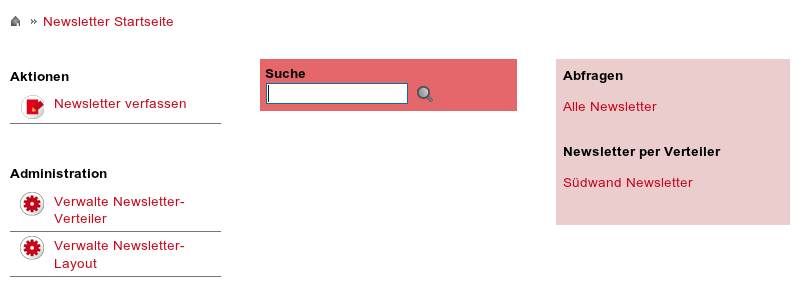
\includegraphics[width=0.9\textwidth]{index}
\caption{Startseite der Newsletter-Verwaltung}
\label{fig:index}
\end{figure}


\section{Newsletter verfassen}

Klicken Sie auf der auf "`Newsletter verfassen"' um einen neuen Newsletter zu erstellen. Alles weitere erfahren Sie im Kapitel \vref{sec:edit}.

\section{Administration - Verwalte Verteiler}

Erstellen und Verwalten der verschiedenen Verteiler. Siehe Kapitel \vref{sec:mailinglists}. 

\section{Administration - Verwalte Layouts}

Erstellen und Verwalten von Layouts für Newsletter. Siehe Kapitel \vref{sec:layouts}. 


\section{Suche}

Durchsucht den Betreff der bisher versandten Newsletter.

Geben Sie eine Suchbegriff oder auch nur einen Teil davon in das Suchfeld ein und drücken Sie $\Enter$ oder klicken Sie das Lupen-Symbol an.

\section{Abfragen}

Öffnen Sie eine Liste aller Newsletter, oder wählen Sie eine Liste eines bestimmten Verteilers. Siehe auch Kapitel \vref{sec:list}.



\chapter{Listenansicht}
\label{sec:list}

In der Listenansicht sehen Sie einen Überblick Ihrer Newsletter.

\begin{figure}[htp]
\centering

\includegraphics[width=0.9\textwidth]{list}
\caption{Liste der Newsletter}
\label{fig:list}
\end{figure}

\section{Filtereinstellungen}

Filter schränken die Anzeige der Listenansicht nach verschiedenen Kriterien ein.

Klicken Sie auf das Papierkorbsymbol eines Filters um es zu entfernen.

\section{Aktionsleiste}

In der Aktionsleiste können Sie einen neuen Newsletter verfassen ("`Erstellen"') oder die die Liste nach gewissen Kriterien filtern bzw. durchsuchen.

Das Suchfeld sucht im Betreff der angezeigten Newsletter.

\section{Liste}

In der Liste selbst sehen Sie die wichtigsten Informationen zum Status der einzelnen Newsletter.

\subsection{Bearbeiten}

Klicken Sie auf das Stiftsymbol um einen Newsletter zu bearbeiten. Siehe hierzu auch Kapitel \vref{sec:edit}.

\subsection{Gesamtanzahl Empfänger}

Zeigt Ihnen die Anzahl der Empfänger. Diese Zahl ergibt sich aus der Summe der Abonnenten der jeweils für den Newsletter ausgewählten Verteiler.

\subsection{Versandt}

Zeigt die Anzahl der Newsletter die tatsächlich versandt wurden. Klicken Sie auf die Zahl um eine Liste aller Empfänger zu sehen.

Falls die Zahl kleiner als die Gesamtanzahl der Empfänger ist, gibt es fehlerhafte E-Mailadressen. Klicken Sie in der gleichen Zeile auf die Zahl der unzustellbaren Newsletter um Näheres über die Fehler herauszufinden.

\subsection{Gelesen}

Hier sehen Sie wieviele Ihrer Empfänger den Newsletter gelesen haben. Klicken Sie auf die Zahl um Details anzuzeigen. Siehe dazu Kapitel \vref{sec:tracking}

Bitte beachten Sie, dass es nicht alle E-Mailprogramme erlauben herauszufinden ob ein Empfänger den Newsletter gelesen hat. Daher ist diese Zahl mit Vorsicht zu genießen.

\subsection{Unzustellbar}

Zeigt wieviele Newsletter unzustellbar waren. Klicken Sie auf die Zahl um Details anzusehen. Details dazu finden Sie im Kapitel \vref{sec:undeliverable}



\chapter{Newsletter verfassen}
\label{sec:edit}

Klicken Sie auf der Newletter-Startseite, oder in der Listenansicht auf "`Erstellen"'.

\begin{figure}[htp]
\centering

\includegraphics[width=0.9\textwidth]{edit}
\caption{Newsletter verfassen}
\label{fig:edit}
\end{figure}

\section{Felder}

\subsection{Verteiler}

Wählen Sie einen oder mehrere Verteiler an den Sie den Newletter senden möchten
Verteiler die in der Verwaltung (siehe Kapitel \vref{sec:verteiler}) als Standardverteiler markiert wurden sind bereits ausgewählt.

\subsection{Betreff}

Geben Sie einen Betreff ein.

\subsection{Text}

Den Inhalt Ihres Newsletter geben Sie im Feld "`Text"' ein. Es steht Ihnen eine WYSIWYG-Editor ähnlich wie von Word oder OpenOffice gewohnt zur Verfügung. Sie können also Überschriften, Aufzählunglisten und Schriftformatierungen wählen. Auch das Einfügen von Links und Bildern ist möglich.

Ausführliche Informationen zum Editor erhalten Sie im Handbuch "`ullCms"'.

Für personalisierte E-Mails können Sie eine Reihe von Platzhaltern verwenden.

Beispiele:
\begin{description}
 % "[" is interpreted -> use \lbrack instead
 % the underscore in ONLINE_LINK is interpreted (!?%&) -> escape with \
 \item[\lbrack FIRST\_NAME\rbrack] Der Vorname des Empfängers
 \item[\lbrack LAST\_NAME\rbrack] Der Nachname des Empfängers
 \item[\lbrack TITLE\rbrack] Der Titel
\end{description}

Beispiel: Hallo [FIRST\_NAME] [LAST\_NAME]!

\subsection{Layout}

Wählen Sie ein Layout aus der Liste. Im Normalfall ist Ihr Standardlayout bereits vor-ausgewählt.

\section{Senden}

Wenn Sie mit dem Verfassen fertig sind, können Sie sich mittels "`Sende Test-Newsletter an mich"' einen Newsletter an Ihre eigene E-Mailadresse zusenden um die Darstellung zu überprüfen

Sind Sie zufrieden senden Sie den Newsletter durch Klick auf "`Sende Newsletter"' ab. Bestätigen dazu die Sicherheitsabfrage.

Sie werden nun zur Listenansicht weitergeleitet und erhalten eine Meldung an wieviele Empfänger der Aufrag zur Sendung des Newsletters entgegengenommen wurde.

Je nach Anzahl der Empfänger kann das Versenden bis zu mehreren Stunden dauern. Sie können jederzeit nachsehen wieviele E-Mails bereits versendet wurden in dem Sie die Listenansicht aktualisieren (Taste [F5]).



\chapter{Verteiler}
\label{sec:verteiler}

Legen Sie Verteiler für jede Zielgruppe an. Sie sprechen so jede Interessentengruppe gezielt an und vermeiden Abmeldungen wegen uniteressanten Informationen für Ihre Kunden.

\section{Verwaltung}

Gehen Sie in den Administrationsbereich ("`Admin"') und wählen Sie "`Verwalte Newsletter Verteiler"'.

\section{Erstellen}
\label{sec:create-mailing-list}

Klicken Sie auf "`Erstellen"'

\subsection{Name}

Geben Sie den Namen für den Verteiler ein.

Beispiel: Produktneuigkeiten für Gemüsehändler

\subsection{Beschreibung}

Beschreiben Sie welche Informationen Ihre Kunden über diesen Verteiler erhalten.

Denken Sie an folgende Punkte:
\begin{itemize}
 \item Zielgruppe
 \item Themen
 \item Anzahl der Newsletter pro Jahr
\end{itemize}

Beispiel:  

Erhalten Sie 4-6 Mal jährlich interessante Produktneuigkeiten und Erfahrungsberichte aus dem Bereich des Gemüsehandels.

\subsection{Automatisch anmelden}

Hier geht es darum ob neu angelegte Benutzer automatisch für den aktuellen Newsletter angemeldet werden.
Dabei ist es egal ob Sie einen Benutzer händisch anlegen oder ob sich der Benutzer selbst auf Ihrer Webseite registriert.

\subsection{Standard-Verteiler}

Wenn Sie dieses Feld anhaken wird beim Verfassen eines neuen Newsletter dieser Verteiler automatisch ausgewählt.

\subsection{Ist aktiv}

Damit steuern Sie ob der aktuelle Verteiler in der Liste Ihrer Verteiler aufscheint.

Wenn dieses Feld nicht angekreuzt wird, können Kunden sich nicht für diesen Verteiler anmelden.


\chapter{Layouts}

Ein Layout ist eine Art Formatvorlage um Ihren Newslettern ein einheitliches und attraktives Aussehen zu verleihen.

Im Normalfall genügt es einmal ein Layout im Stile Ihrer CI (Corporate Identity) anzulegen.

Sie können beliebig viele Layouts anlegen.


\section{Verwaltung}

Gehen Sie in den Administrationsbereich ("`Admin"') und wählen Sie "`Verwalte Newsletter Layouts"'.

\section{Erstellen}
\label{sec:create-layout}

Klicken Sie auf "`Erstellen"'

\subsection{Name}

Geben Sie einen Namen für das neue Layout ein. Beispiel: "`Standard"'

\subsection{HTML-Head}

Der "`head"' Teil des HTML Codes. Hier können Sie z.B. CSS Stylesheet Anweisungen einfügen.

Beispiel:

\begin{lstlisting}
<style type="text/css">
  body {
    font-size 10pt; 
  }
  
  h1 { 
    color: red;
  } 
</style>
\end{lstlisting}

Hinweis: Der "`<head>"' Tag ist nicht erforderlich.

\subsection{HTML-Body}

Geben Sie hier den HTML-Code für Ihr Layout ein.

Sie können den grafischen WYSIWYG (What you see is what you get) Editor verwenden oder durck Klick auf den Button "`Quellcode"' zum HTML-Code umschalten.

Tips und Tricks zur Verwendung des Editors erhalten Sie im ullCms Handbuch.


Folgende Platzhalter stehen zur Verfügung:

\begin{description}
 % "[" is interpreted -> use \lbrack instead
 % the underscore in ONLINE_LINK is interpreted (!?%&) -> escape with \
 \item[\lbrack ONLINE\_LINK\rbrack] Fügt den Link zur Online-Version des Newsletters ein ("`Haben Sie Probleme mit der Ansicht des Newsletters klicken Sie hier..."')
 \item[\lbrack CONTENT\rbrack] Platzhalter für den eigentlichen Inhalt des Newsletters
 \item[\lbrack UNSUBSCRIBE\rbrack] Fügt die Unsubscribe-Links zur Abmeldung ein
 \item[\lbrack TRACKING\rbrack] Fügt die Funktionalität für das Tracking ein ("`Wer hat den Newsletter gelesen"')
\end{description}


Ein einfaches Beispiel:

\begin{lstlisting}
<h1>ullright Product News</h1>

<p>[ONLINE_LINK]<p>

<p>[CONTENT]</p>

<p>[UNSUBSCRIBE]</p>
<p>(C) 2011 by ull.at</p>
\end{lstlisting}

\subsection{Ist Standardlayout}

Wenn Sie dieses Feld anhaken wird dieses Layout beim Verfassen eines neuen Newsletter automatisch vor-ausgewählt.

\section{Bearbeiten}

Klicken Sie in der Liste der Layouts auf das Stiftsymbol vor dem Eintrag den Sie bearbeiten möchte.

Alles weitere erfahren Sie im Kapitel \vref{sec:create-layout}.



\end{document}